\documentclass{beamer}
\usepackage[english,russian]{babel}
\usepackage[utf8]{inputenc}
\usepackage{pagenumber}

\usepackage{hyperref}
% Стиль презентации
\usetheme[numbers, totalnumbers]{Dresden}
% цветовая схема
\usecolortheme{beaver}

\makeatletter
\defbeamertemplate*{footline}{Dresden}{
	\leavevmode%
	\hbox{%
	\begin{beamercolorbox}[wd=.3\paperwidth,ht=3.00ex,dp=1ex,center]{author in head/foot}%
		\usebeamerfont{author in head/foot}%
		\insertauthor	
	\end{beamercolorbox}%
	\begin{beamercolorbox}[wd=0.5\paperwidth,ht=3.00ex,dp=1ex,center]{title in head/foot}%
		\usebeamerfont{title in head/foot}\inserttitle
	\end{beamercolorbox}%
	\begin{beamercolorbox}[wd=.2\paperwidth,ht=3.00ex,dp=1ex,right]{date in head/foot}%
		\usebeamerfont{date in head/foot}\hspace*{2em}
		\insertframenumber{} / \inserttotalframenumber\hspace*{2ex}
	\end{beamercolorbox}}%
}
\makeatother

\begin{document}
\title{Linux Kernel Networking}  
\author{Волков Д., Заславский М.}
\institute{Computer Science Center}
\date{\today} 

% -- Представление, приветы
\frame{\titlepage} 

% -- В рамках этого проекта я работал в основном над улучшением
% -- системы проверки вот этого курса на stepic, поднимите ваши
% -- руки, кто с этим курсом знаком (если кто-то поднял, то ещё
% -- поднимите кто прошел этот курс). Спросить, если ненулевые
% -- количества поднятых рук, долго ли приходилось ожидать про-
% -- верки задач.
\begin{frame}{Stepic}
	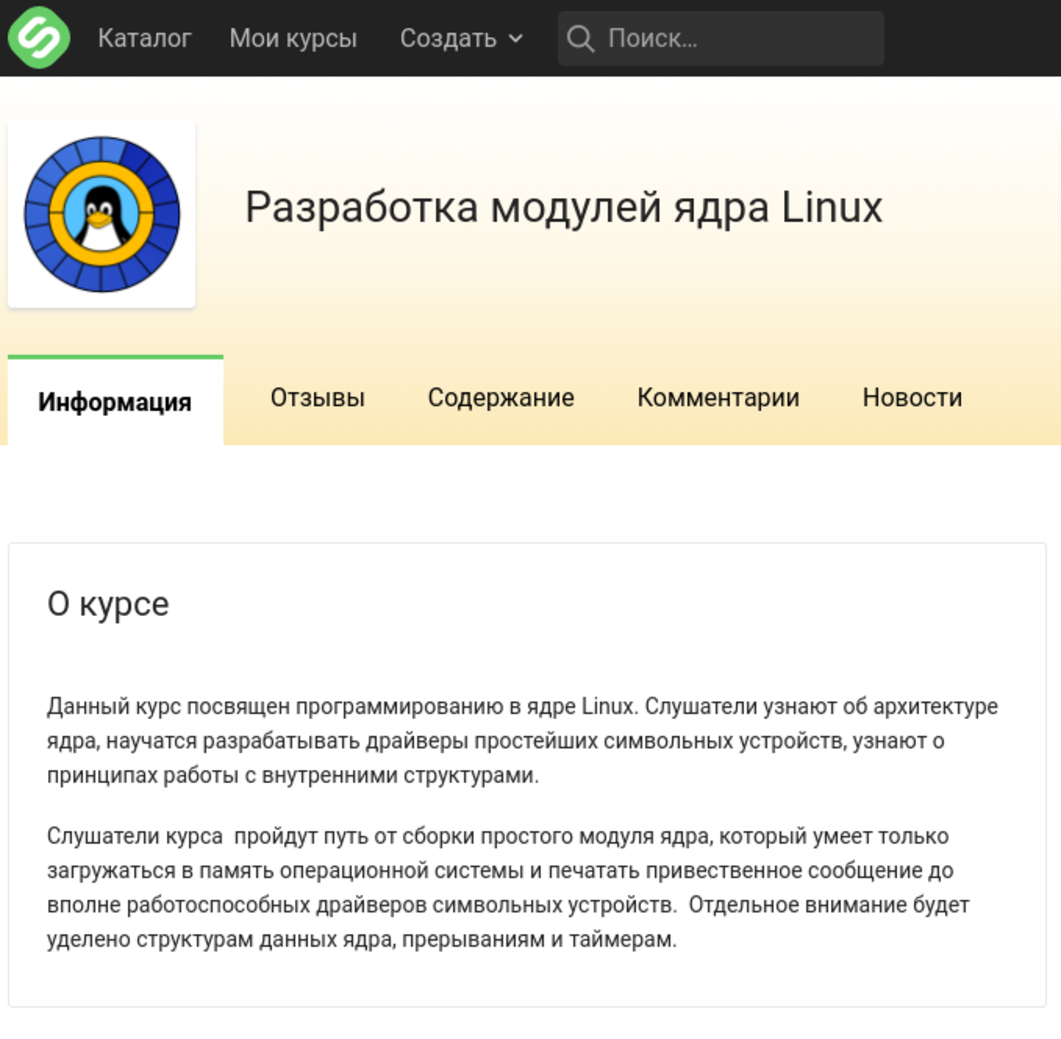
\includegraphics[width=100mm]{./stepic.pdf}
\end{frame}

% -- Более формальный слайд, представляющий цели и задачи проекта.
% -- Каждая задача непосредственно вытекает из потребностей, сфор-
% -- мулированный выше.
\begin{frame}{Цели и задачи}
	\textbf{Цель проекта:} 
        Создание задач для нового модуля в курсе (ссылка), посвященного работе с сетевым стеком Linux.
	\textbf{Задачи:}
	\begin{itemize}
		\item Знакомство с сетевыми технологиями 
		\item Знакомство с сетевым стеком Linux
		\item Создание концепций задач и плана их проверки
		\item Реализация в проверящей системе проверки задач
	\end{itemize}
\end{frame}

% -- слайд про сетевой стек
\begin{frame}{Сетевой стек}
\end{frame}

% -- В существующим курсе занимает довольно далекое от начала место 
\begin{frame}{Новый модуль}
	\begin{itemize}
		\item Знакомство с API сетевого стека ядра
		\item Сетевые интерфейсы и работа с ними
		\item Подсистема ядра Netlink
		\item Пользовательские сетевые протоколы различных уровней
		\item Реализация какого-нибудь своего протокола
	\end{itemize}
\end{frame}

\begin{frame}{Обзор новых задач}
	\begin{itemize}
		\item В первой задаче мы просим пользователя вывесте некоторые внутренние данные сетевых устройств Linux.
	\end{itemize}
\end{frame}


\begin{frame}{Обзор новых задач}
	\begin{itemize}
		\item В первой задаче мы просим пользователя вывесте некоторые внутренние данные сетевых устройств Linux.
		\item Нужно создать сетевое устройство в системе, с заданными параметрами.
	\end{itemize}
\end{frame}

\begin{frame}{Обзор новых задач}
	\begin{itemize}
		\item В первой задаче мы просим пользователя вывесте некоторые внутренние данные сетевых устройств Linux.
		\item Нужно создать сетевое устройство в системе, с заданными параметрами.
		\item Нужно, чтобы подобных сетевых устройств было несколько, в заданной иерархии и заданного типа.
	\end{itemize}
\end{frame}

\begin{frame}{Обзор новых задач}
	\begin{itemize}
		\item В первой задаче мы просим пользователя вывесте некоторые внутренние данные сетевых устройств Linux.
		\item Нужно создать сетевое устройство в системе, с заданными параметрами.
		\item Нужно, чтобы подобных сетевых устройств было несколько, в заданной иерархии и заданного типа.
		\item Далее, наше сетевое устройство теперь должно перехватывать трафик определенного типа и извлекать из него информацию.
	\end{itemize}
\end{frame}

\begin{frame}{Обзор новых задач}
	\begin{itemize}
		\item В первой задаче мы просим пользователя вывесте некоторые внутренние данные сетевых устройств Linux.
		\item Нужно создать сетевое устройство в системе, с заданными параметрами.
		\item Нужно, чтобы подобных сетевых устройств было несколько, в заданной иерархии и заданного типа.
		\item Далее, наше сетевое устройство теперь должно перехватывать трафик определенного типа и извлекать из него информацию.
		\item Помимо извлечения информации, неплохо было бы передавать её на другой интерфейс, либо отсылать на определенный адрес в сети, или что-то подобное.
	\end{itemize}
\end{frame}
\begin{frame}{Обзор новых задач}
	\begin{itemize}
                \item Собственно, на этом этапе мы уже готовы реализовать какой-нибудь стандартный протокол маршрутизации (но лучше учебный, облегченного варианта)
	\end{itemize}
\end{frame}


% -- слайд про сетевой стек
\begin{frame}{Сетевой стек}
\end{frame}

% -- В рамках этого проекта мне удалось поработать со следующими тех-
% -- нологиями (небольшое перечисление с коментариями по ходу)
\begin{frame}{Технологии}
        Использовались:
	\begin{itemize}
		\item OC: \textbf{Linux}
		\item Языки: \textbf{С}, \textbf{Bash}
		\item Система контроля версий: \textbf{Git}
	\end{itemize}
\end{frame}

% -- Резюмируя
\begin{frame}{Результаты}
        Что будет знать и уметь студент курса, осиливший этот модуль:
	\begin{itemize}
		\item Понимать, о чем идет речь, читая исходники ядра
		\item Путь пакета в ядре от физического устройства до приложения
		\item Как написать свой перехватчик трафика
		\item Как реализованы те или иные протоколы в ядре
		\item Как реализовать при необходимости свой
                \item Как написать свой маршрутизатор (?)
	\end{itemize}
\end{frame}

\begin{frame}{Перспективы}
	Направления для развития:
	\begin{itemize}
                \item Сделать более гладким переход от легких задач модуля к тяжелым (?)
                \item Сделать теоретическую часть модуля
	\end{itemize}
\end{frame}

% -- Ссылка на тот самый курс
\begin{frame}{Ссылки}
	\begin{itemize}
		\item Курс: \textbf{https://stepik.org/course/2051}
	\end{itemize}
\end{frame}

\begin{frame}{Emails}
	\begin{itemize}
		\item Волков Д. \textbf{volkov12@rambler.ru}
		\item Заславский М. \textbf{mark.zaslavskiy@gmail.com}
	\end{itemize}
\end{frame}

\begin{frame}{Ссылки}
	\begin{itemize}
		\item \textbf{https://github.com/cscenter/mooc-linux-programming}
	\end{itemize}
\end{frame}

\end{document}
